

\chapter{LES models with Algo\_QC in \texttt{TrioCFD}}
\lhead{Quasi compressible highly anisothermal turbulence}
\section{Solved equations}
The Algo\_QC module in \texttt{TrioCFD} implementes the low mach number equations in the context of quasi compressible equations, aswell as many Thermal-Large Eddy Simulation (T-LES) models.  This approximation aims to narrow the gap between incompressible and compressible Navier-Stokes equations and is suitable for the computation of convection in a fluid in the presence of large density gradients \cite{paolucci_filtering_1982}. The low Mach number equations consider internal wave propagation, but they do not take into account acoustic waves. Thus, the numerical methods developed for incompressible flow can be used. This approximation conducts to divide the pressure into two terms: the thermodynamical pressure which is homogeneous and the mechanical pressure. The Stokes hypothesis is assumed to be true \cite{Papalexandris2019}. The solved equations are the following:



\begin{itemize}
    \item Mass conservation equation
        \begin{equation}
            \frac{\partial \rho}{\partial t} + \frac{\partial \rho U_j}{\partial x_j} = 0
            \label{eq:mass_conserv}
        \end{equation}
    
    \item Momentum conversation equation
    \begin{equation}
        \frac{
            \partial \rho U_i
        }{
            \partial t
        } = - \frac{
            \partial \rho U_j U_i
        }{
            \partial x_j
        } - \frac{\partial P}{\partial x_i} + \frac{\partial \Sigma_{ij}(U, T)}{\partial x_j}
        \label{eq:moment_conserv}
    \end{equation}
    
    \item Energy conservation equation
    \begin{equation}
        \frac{
            \partial
        }{
            \partial x_j
        } U_j = - \frac{1}{\gamma P_0} \Big[  (\gamma -1) \Big( \frac{\partial Q_j }{\partial x_j} \Big) + \frac{\diff P_0}{\diff t}\Big]
        \label{eq:ener_conserv}
    \end{equation}
    
    \item Ideal gas law
    \begin{equation}
        T = \frac{P_0}{\rho r}
        \label{eq:ideal_gas}
    \end{equation}
    With $\rho$ density, $T$ temperature, $\gamma$ the heat capacity, $r=287 \ \text{J} \cdot \text{kg}^{-1} \cdot \text{K}^{-1}$
\end{itemize}

with $t$ the time, $P$ the mechanical pressure, $P_0$ thermo dynamical pressure, $U_i$ the $i^{\text{th}}$ component of velocity, and $x_i$ the Cartesian coordinate in the $i^{\text{th}}$ direction. The Einstein summation convention is employed. The thermodynamical pressure is obtained by integrating Equation~\ref{eq:ener_conserv} over the volume of the studied geometry:

\begin{equation}
    \difffrac{P_0}{t} = -(\gamma -1) \Big( \frac{1}{V} \int Q_j({T}) \diff S_j \Big)
\end{equation}
With V the volume of the computational domain and $S_j$ the boundaries of the investigated domain.

The shear-stress tensor and the conductive heat flux are respectively computed with the functions $\Sigma_{ij}({U}, {T})$ and $Q_j({T})$, assuming Newtonian fluid and Fourier's law, leading to the following expressions:

\begin{equation}
    \Sigma_{ij}({U}, {T}) = \mu ({T}) \Big( \pfrac{{U_i}}{x_j} + \pfrac{{U_j}}{x_i}\Big) - \frac{2}{3}\mu({T}) \pfrac{{U_k}}{x_k} \delta_{ij}
\end{equation}

\begin{equation}
    Q_j({T}) = - \lambda({T})\pfrac{{T}}{x_j}
\end{equation}

where $\mu(T)$ is the dynamic viscosity, $\lambda(T)$ is the thermal conductivity, and $\delta_{ij}$ the Kronecker symbol.
The fluid passing through the channel is air. Sutherland's law \cite{sutherland_viscosity_1893} is used to compute viscosity from temperature:

\begin{equation}
    \mu(T) = \mu_0 \frac{T}{T_0}^{3/2} \frac{T_0 + S}{T + S}
\end{equation}

where $\mu_0 = 1.716 \times 10^{-5} \ \text{Pa}\cdot\text{s}$, $S = 110.4 \ \text{K}$, and $T_0 = 273.15 \ \text{K}$. The Prandtl number is assumed to be constant in this simulation, and the heat capacity at constant pressure $C_p$ is obtained with the average of wall temperatures. The conductivity is deduced from the Prandtl number, the heat capacity at constant pressure, and the viscosity.

\begin{equation}
    \lambda(T) = \frac{C_p}{P_r} \mu(T)
\end{equation}

\begin{figure}
  \begin{center}
    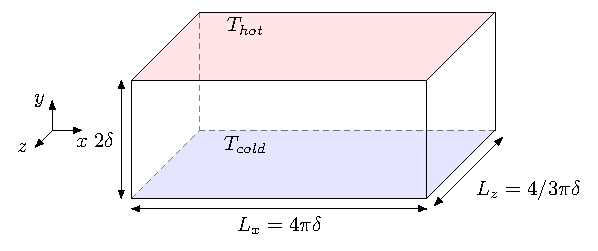
\includegraphics[width=0.95\textwidth]{./figures/canal_plan.pdf}
  \end{center}
  \caption{}
  \label{figure:canal_plan_anisotherme}
\end{figure}


We suppose two boundary temperatures $T_{\text{hot}}$ and $T_{\text{cold}}$, where the temperature differense is of the order of $300K$ to $400K$, with figure~\ref{figure:canal_plan_anisotherme} as a representation.
The streamwise ($x$) and spanwise directions ($z$) are periodic.

A hyperbolic tangent mesh is used in the wall-normal direction ($y$).

The wall-normal grid coordinates are symmetrical with respect to the plane $y=h$. In the first half of the channel, they are given by
\begin{equation}
y_k = h \left( 1 + \frac{1}{a} \tanh\left[ \left(\frac{k-1}{N_y-1} - 1\right)\tanh^{-1}(a)\right] \right), \label{eqmesh}
\end{equation}

with $a$ the mesh dilatation parameter.

\section{Filtered low Mach number equations}\label{label-pa}

We consider the large-eddy simulation of the
low Mach number equations in two formulations as introduced in \cite{dupuy2018study}. The Velocity formulation
expresses the filtered low Mach number equations in terms of variables
filtered with the unweighted classical filter ($\overline{\,\,\cdot\,\,}$).
The Favre formulation expresses the filtered low Mach number equations using
Favre-filtered variables,
that is based on the density-weighted Favre filter ($\fa{\,\,\,\cdot\,\,}$)
defined for any field~$\psi$ as $\fa{\psi} = \f{\rho \psi} / \f{\rho}$.
The two formulations involve a different set of subgrid terms.
However, the two most significant subgrid terms are similar in the two
formulations \cite{dupuy2016, dupuy2017sft, dupuy2018study}.
In both cases, a subgrid term is related to the nonlinearity of momentum
convection and another related to the correlation of density and velocity.
Excluding all other subgrid terms, the filtered low Mach number equations are
given in the Velocity formulation by:
\begin{itemize}
\item Mass conservation equation
\begin{equation}
\der{\f{\rho}}{t} + \der{}{x_j}\left(\f{\rho} \f{U}_{\!j} + F_{\rho U_j}\right) = 0,
\end{equation}
\item Velocity transport equation
\begin{equation}
\begin{aligned}
\der{\f{U}_{\!i}}{t} = - \der{\left(\smash[t]{\f{U}_{\!j} \f{U}_{\!i} + F_{U_j U_i}}\right)}{x_j} + \f{U}_{\!i} \der{\f{U}_{\!j}}{x_j} - \frac{1}{\f{\rho}}\der{\f{P}}{x_i} + \frac{1}{\f{\rho}} \der{\varSigma_{ij}(\vv{\f{U}}, \f{T})}{x_j},
\end{aligned}
\end{equation}
\item Energy conservation equation
\begin{equation}
\der{\f{U}_{\!j}}{x_j} = - \frac{1}{\gamma P_{0}}\left[ (\gamma - 1)\der{Q_j(\f{T})}{x_j} + \der{P_{0}}{t} \right],
\end{equation}
\item Ideal gas law
\begin{equation}
\f{T} = \frac{P_{0}}{r \f{\rho}},
\end{equation}
\end{itemize}
and in the Favre formulation by:
\begin{itemize}
\item Mass conservation equation
\begin{equation}
\der{\f{\rho}}{t} + \der{\f{\rho} \fa{U_{j}}}{x_j} = 0,
\end{equation}
\item Momentum conservation equation
\begin{equation}
\begin{aligned}
\der{\f{\rho} \fa{U}_{\!i}}{t} = - \der{\left(\smash[t]{\f{\rho} \fa{U}_{\!j} \fa{U}_{\!i} + \f{\rho} G_{U_j U_i}}\right)}{x_j} - \der{\f{P}}{x_i} + \der{\varSigma_{ij}(\vv{\fa{U}},\fa{T})}{x_j},
\end{aligned}
\end{equation}
\item Energy conservation equation
\begin{equation}
\der{}{x_j}\left(\fa{U}_{\!j} + \f{\rho} G_{U_j/\rho}\right) = - \frac{1}{\gamma P_{0}}\left[ (\gamma - 1)\der{Q_j(\fa{T})}{x_j} + \der{P_{0}}{t} \right],
\end{equation}
\item Ideal gas law
\begin{equation}
\fa{T} = \frac{P_{0}}{\f{\rho} r},
\end{equation}
\end{itemize}
with $\rho$ the density, $T$ the temperature, $\gamma$ the heat capacity ratio,
$r$ the ideal gas specific constant, $t$ the time, $P$ the mechanical pressure,
$P_0$ the thermodynamical pressure, $U_i$ the $i$-th component of velocity and
$x_i$ the Cartesian coordinate in $i$-th direction. Einstein summation
convention is used.
The functions $\varSigma_{ij}(\vv{U}, T)$ and $Q_j(T)$ are used to compute the
shear-stress tensor and conductive heat flux associated with a given velocity
and temperature. We assume a Newtonian fluid
and Fourier's law,
\begin{align}
\varSigma_{ij}(\vv{U}, T) ={}& \mu(T) \left(\der{U_i}{x_j} + \der{U_j}{x_i}\right) - \frac{2}{3} \mu(T) \der{U_k}{x_k} \delta_{ij}, \\
Q_j(T) {}&= - \lambda(T) \der{T}{x_j},
\end{align}
with $\mu(T)$ the dynamic viscosity, $\lambda(T)$ the thermal conductivity and
$\delta_{ij}$ the Kronecker delta.

The momentum convection subgrid term is defined as
$\smash[t]{F_{U_j U_i} ={} \f{U_j U_i} - \f{U}_{\!j} \f{U}_{\!i}}$ in the Velocity formulation and
$\smash[t]{G_{U_j U_i} ={} \fa{U_j U_i} - \fa{U}_{\!j} \fa{U}_{\!i}}$ in the Favre formulation.
The density-velocity correlation subgrid term is defined as
$\smash[t]{F_{\rho U_j} ={} \f{\rho U_j} - \f{\rho} \f{U}_{\!j}}$ in the Velocity formulation and
$\smash[t]{G_{U_j/\rho} ={} \fa{U_j/\rho} - \fa{U}_{\!j}/\f{\rho}}$ in the Favre formulation.
The two formulations are related by the relation
\begin{equation}
\frac{F_{\rho U_j}}{\f{\rho}} = - \f{\rho} G_{U_j/\rho}.
\end{equation}



The fluid is air. We use Sutherland's law \cite{sutherland1893lii} to compute the viscosity,
\begin{equation}
\mu(T) = \mu_0 \left(\frac{T}{T_0}\right)^{\frac{3}{2}} \frac{T_0 + S}{T + S},
\end{equation}
with $\mu_0 = 1.716\cdot 10^{-5}$~Pa~s, $S=110.4$~K and $T_0 = 273.15$~K.
We assume a constant Prandtl number $Pr = 0.76$ and heat capacity at
constant pressure $C_p~=~1005$~J~kg$^{-1}$~K$^{-1}$.
The conductivity is deduced from the Prandlt number, the heat capacity at
constant pressure and the viscosity,
\begin{equation}
\lambda(T) = \frac{C_p}{Pr} \mu(T).
\end{equation}
The ideal gas specific constant is~$r=287$~J~kg$^{-1}$~K$^{-1}$.


These equations can be solved through the keywork \texttt{large\_eddy\_simulation\_formulation}, with either the \texttt{favre} or \texttt{velocity} values.

the following section is directly taken from~\cite{dupuy2016,dupuy2017sft,dupuy2018study}.

\section{Subgrid-scale models}

The subgrid terms of the Velocity and Favre formulations are formally
similar. Accordingly, the same modelling procedure is used in both cases.
To formalise this, we may express the subgrid-scale models as a function
of the filter length scales and of the filtered velocity and density
in the two formulations:
\begin{align}
F_{U_j U_i} \approx{}& \tau_{ij}^{\mathrm{mod}}(\vv{\f{U}}, \vv{\f{\Delta}}), \\
G_{U_j U_i} \approx{}& \tau_{ij}^{\mathrm{mod}}(\vv{\fa{U}}, \vv{\f{\Delta}}), \\
F_{\rho U_j} \approx{}& \pi_{j}^{\mathrm{mod}}(\vv{\f{U}}, \f{\rho}, \vv{\f{\Delta}}), \\
G_{U_j/\rho} \approx{}& \pi_{j}^{\mathrm{mod}}(\vv{\fa{U}}, 1/\f{\rho}, \vv{\f{\Delta}}),
\end{align}%
where the functions $\tau_{ij}^{\mathrm{mod}}(\vv{U},\vv{\f{\Delta}})$ and
$\pi_j^{\mathrm{mod}}(\vv{U},\phi,\vv{\f{\Delta}})$ are model-dependent but do not depend on the formulation.

Eddy-viscosity models for the subgrid term associated with momentum convection
may be written in the form
\begin{align}
\tau_{ij}^{\mathrm{mod}}(\vv{U}, \vv{\f{\Delta}}) ={}& - 2 \nu_e^{\mathrm{mod}}(\vv{g}, \vv{\f{\Delta}}) S_{ij}, \label{hela}
\end{align}%
with
$S_{ij} = \tfrac{1}{2}\left( g_{ij} + g_{ji} \right)$ the rate of deformation tensor
and
$\vv{g}$
the velocity gradient, defined by $g_{ij} = \partial_j U_i$.
Notice that $\tau_{ij}^{\mathrm{mod}}(\vv{U}, \vv{\f{\Delta}})$ may be
considered traceless without loss of generality, even in the incompressible case,
since the trace can be included as part of the filtered pressure $\f{P}$.
The eddy-viscosity $\nu_e^{\mathrm{mod}}(\vv{g}, \vv{\f{\Delta}})$
is given by the model used.
The following models from the literature are investigated in this paper using a priori tests:
\begin{flalign}
&\textrm{Smagorinsky model \cite{smagorinsky1963general}:} & \nu_e^{\mathrm{Smag.}}  (\vv{g}, \vv{\f{\Delta}}) ={}& \left( C^{\mathrm{Smag.}} \f{\Delta} \right)^2 \left|\vt{S}\right|, &&& \label{sma} \\
&\textrm{WALE model \cite{nicoud99b}:}                     & \nu_e^{\mathrm{WALE}}   (\vv{g}, \vv{\f{\Delta}}) ={}& \left( C^{\mathrm{WALE}} \f{\Delta} \right)^2 \frac{\left(\mathcal{S}^d_{ij} \mathcal{S}^d_{ij}\right)^{\tfrac{3}{2}}}{\left(S_{mn} S_{mn}\right)^{\tfrac{5}{2}} + \left(\mathcal{S}^d_{mn} \mathcal{S}^d_{mn}\right)^{\tfrac{5}{4}}}, &&& \\
&\textrm{Vreman model \cite{vreman2004eddy}:}              & \nu_e^{\mathrm{Vreman}} (\vv{g}, \vv{\f{\Delta}}) ={}& C^{\mathrm{Vreman}} \sqrt{\frac{\mathrm{II}_G}{g_{mn}g_{mn}}}, &&& \\
&\textrm{Sigma model \cite{nicoud2011using}:}              & \nu_e^{\mathrm{Sigma}}  (\vv{g}, \vv{\f{\Delta}}) ={}& \left( C^{\mathrm{Sigma}} \f{\Delta} \right)^2 \frac{\sigma_3\left(\sigma_1 - \sigma_2\right)\left(\sigma_2 - \sigma_3\right)}{\sigma_1^2}, &&& \\
&\textrm{AMD model \cite{rozema2015minimum}:}              & \nu_e^{\mathrm{AMD}}    (\vv{g}, \vv{\f{\Delta}}) ={}& C^{\mathrm{AMD}} \frac{\max(0, - G_{ij} S_{ij})}{g_{mn}g_{mn}}, &&& \\
&\textrm{VSS model \cite{ryu2014subgrid}:}                 & \nu_e^{\mathrm{VSS}}    (\vv{g}, \vv{\f{\Delta}}) ={}& \left( C^{\mathrm{VSS}} \f{\Delta} \right)^2  \frac{\left(R_{ij} R_{ij}\right)^{\frac{3}{2}}}{\left(S_{mn}S_{mn}\right)^{\frac{5}{2}}}, &&& \\
&\textrm{Kobayashi model \cite{kobayashi2005subgrid}:}     & \nu_e^{\mathrm{Koba.}}  (\vv{g}, \vv{\f{\Delta}}) ={}& C^{\mathrm{Koba.}} \f{\Delta}^2 \left|F_g\right|^{\frac{3}{2}} (1-F_g) \left|\vt{S}\right|, &&& \label{koba}
\end{flalign}%
where 
$\left|\vt{S}\right|=\sqrt{2 S_{ij} S_{ij}}$ is a norm of $\vt{S}$,
$\mathcal{S}^d_{ij} = \tfrac{1}{2}\left( g_{ik}g_{kj} + g_{jk}g_{ki} \right) - \tfrac{1}{3}g_{kp}g_{pk} \delta_{ij}$ the traceless symmetric part of the squared velocity gradient tensor, 
$\sigma_1 \geq \sigma_2 \geq \sigma_3$ the three singular values of $\vv{g}$,
$G_{ij} = \f{\Delta}_k^2 g_{ik} g_{jk}$ the gradient model for the subgrid term associated with momentum convection \cite{leonard74},
$\mathrm{II}_G = \tfrac{1}{2}\left(\tr^2\left(G\right) - \tr\left(G^2\right)\right)$ its second invariant,
$R_{ij}=\beta_i g_{jj}$ the volumetric strain-stretching, with $\beta=\left(S_{23}, S_{13}, S_{12}\right)$,
and $F_g = \left(\varOmega_{ij}\varOmega_{ij} - S_{ij}S_{ij}\right)/\left(\varOmega_{mn}\varOmega_{mn} + S_{mn}S_{mn}\right)$
the coherent structure function, with $\varOmega_{ij} = \tfrac{1}{2}\left( g_{ij} - g_{ji} \right)$ the spin tensor or rate of rotation tensor.
Only constant coefficient versions of eddy-viscosity and eddy-diffusivity models are considered.
The typical value of the coefficients from the literature is
$C^{\mathrm{Smag.}} = 0.10$, $C^{\mathrm{WALE}} = 0.55$, $C^{\mathrm{Vreman}}=0.07$, $C^{\mathrm{Sigma}}=1.5$, $C^{\mathrm{AMD}}=0.3$, $C^{\mathrm{VSS}}=1.3$ and $C^{\mathrm{Koba.}}=0.045$.
The corresponding dynamic versions of these models are not considered
in order to assess the relevance of the models before any dynamic correction \cite{germano91, lilly1992proposed, park2006dynamic}.
The filter length scale is computed following \cite{deardorff1970numerical} as  $\f{\Delta}=(\f{\Delta}_x\f{\Delta}_y\f{\Delta}_z)^{1/3}$.
A review of alternative possible definitions may be found in \cite{trias2017new}.

Following the same rationale, eddy-diffusivity models for the density-velocity
correlation subgrid term may be written in the form
\begin{align}
\pi_{j}^{\mathrm{mod}}(\vv{U}, \phi, \vv{\f{\Delta}}) ={}& - 2 \kappa_e^{\mathrm{mod}}(\vv{g}, \vv{d}, \vv{\f{\Delta}}) d_j. \label{helb}
\end{align}%
with $\vv{d}$
the scalar gradient, defined by $d_{j} = \partial_j \phi$.
It is common to express the eddy-diffusivity $\kappa_e^{\mathrm{mod}}(\vv{g}, \vv{\f{\Delta}})$
using the constant subgrid-scale Prandtl or Schmidt number assumption,
\begin{align}
\kappa_e^{\mathrm{mod}}    (\vv{g}, \vv{d}, \vv{\f{\Delta}}) ={}& \frac{1}{Pr_t} \nu_e^{\mathrm{mod}}    (\vv{g}, \vv{\f{\Delta}}), \label{dfv}
\end{align}%
where $Pr_t$ is the subgrid-scale Prandtl or Schmidt number. 
This provide a corresponding eddy-diffusivity model for each eddy-viscosity of equations (\ref{sma}--\ref{koba}).
The dimensionless number $Pr_t$ corresponds to a subgrid-scale Schmidt number
in the Velocity formulation and a subgrid-scale Prandtl number in the Favre
formulation.
Given the formal similarity between the density-velocity correlation subgrid
term in the Velocity and Favre formulation and the ideal gas law
(\ref{idealgaslawn}) which relates density and temperature, it is presumed that
the same value may be used in the two formulations.
Alternatively, some specific eddy-diffusivity models have been suggested in
the literature \cite{ghaisas2014priori, abkar2016minimum}.
We investigate using a priori tests the eddy-diffusivity models associated with equations (\ref{sma}--\ref{koba}) and the following specific model:
\begin{flalign}
&\textrm{Scalar AMD model \cite{abkar2016minimum}:}        & \kappa_e^{\mathrm{SAMD}}   (\vv{g}, \vv{d}, \vv{\f{\Delta}}) ={}& C^{\mathrm{SAMD}} \frac{\max(0, - D_j d_j)}{d_m d_m}, &&&
\end{flalign}%
with $D_j = \f{\Delta}_k^2 g_{jk} d_k$ the gradient model for the density-velocity correlation subgrid term.

In addition, we devised two new eddy-viscosity and eddy-diffusivity models
for the purpose of this study.
First, the Anisotropic Smagorinsky model is a modified version of the Smagorinsky model,
associated with a single
filter length scale, devised to involve the three filter length scales.
This aims to improve the anisotropy of the model.
The model is obtained by substituting in equations
(\ref{hela}) and (\ref{helb}) the velocity gradient $\vv{g}$
 and respectively the scalar
gradient $\vv{d}$
by the
scaled velocity gradient $\vv{g^a}$, defined by $g^a_{ij} = (\f{\Delta}_j/\f{\Delta}) \partial_j U_i$,
and respectively
the scaled scalar gradient $\vv{d^a}$, defined by $d^a_j = (\f{\Delta}_j/\f{\Delta}) \partial_j \phi$.
Namely,
\begin{align}
\tau_{ij}^{\mathrm{An. Smag.}}(\vv{U}, \vv{\f{\Delta}}) ={}& - 2 \nu_e^{\mathrm{Smag.}}(\vv{g^a}, \vv{\f{\Delta}}) S^a_{ij}, \\
\pi_{j}^{\mathrm{An. Smag.}}(\vv{U}, \phi, \vv{\f{\Delta}}) ={}& - 2 \kappa_e^{\mathrm{Smag.}}(\vv{g^a}, \vv{d^a}, \vv{\f{\Delta}}) d^a_j,
\end{align}
with $S^a_{ij} = \tfrac{1}{2}\left( g^a_{ij} + g^a_{ji} \right)$ the scaled rate of deformation tensor.
The eddy-viscosity and eddy-diffusivity are computed using equations (\ref{sma}) and (\ref{dfv}).
A similar procedure could be applied to obtain an anisotropic version
of the
WALE,
Sigma,
VSS and
Kobayashi models.

Besides, we study the multiplicative mixed model based on the gradient model (MMG model), a functional model constructed such that
its magnitude is determined by the gradient model \cite{leonard74} and
its orientation is aligned with the rate of deformation tensor or the scalar
gradient depending on the subgrid term.
This procedure is reminiscent of the multiplicative mixed model
of \cite{ghaisas2014priori, ghaisas2016dynamic} which had an opposite purpose.
The eddy-viscosity and eddy-diffusivity according to the MMG model are given
by,
\begin{flalign}
&\textrm{MMG model:}                     & \nu_e^{\mathrm{MMG}}     (\vv{g}, \vv{\f{\Delta}})         ={}& - C^{\mathrm{MMG}} \frac{G_{kk}}{\left|\vt{S}\right|}, &&& \\
&\textrm{Scalar MMG model:}              & \kappa_e^{\mathrm{SMMG}} (\vv{g}, \vv{d}, \vv{\f{\Delta}}) ={}& - C^{\mathrm{SMMG}} \frac{\sqrt{D_i D_i}}{\sqrt{d_m d_m}}. &&&
\end{flalign}%
A similar procedure can be applied to other structural
models, such as the scale-similarity model \cite{bardina1980improved}.
We may also view the MMG model as a multiplicative mixed model. 
Using the the Smagorinsky model and the isotropic part modelling of
\cite{yoshizawa1986statistical},
\begin{align}
\tau_{mm}^{\mathrm{Yosh.}}(\vv{U}, \vv{\f{\Delta}}) ={}& 2 C^{\mathrm{Yosh.}} \f{\Delta}^2 \left|\vt{S}\right|^2,
\end{align}
the MMG model $\tau_{ij}^{\mathrm{MMG}}(\vv{U}, \vv{\f{\Delta}}) = - 2 \nu_e^{\mathrm{MMG}}(\vv{g}, \vv{\f{\Delta}}) S_{ij}$
can be reformulated as
\begin{align}
\tau_{ij}^{\mathrm{MMG}}(\vv{U}, \vv{\f{\Delta}}) ={}& G_{kk}\frac{ \tau_{ij}^{\mathrm{Smag.}}(\vv{U}, \vv{\f{\Delta}})}{\tau_{mm}^{\mathrm{Yosh.}}(\vv{U}, \vv{\f{\Delta}})}
 %
\end{align}
emphasising that the MMG model combines the magnitude of the gradient model
and the structure of the Smagorinsky model.
This leads by identification $C^{\mathrm{MMG}} = (C^{\mathrm{Smag.}})^2/(2C^{\mathrm{Yosh.}})$.
Note that the Vreman, AMD and scalar AMD models also directly involve the gradient model \cite{leonard74}. 


Keywords for most LES models include

\texttt{turbulent\_viscosity} $\tau^{mod}(\overline{U}, \overline{\Delta}) \approx R_{ij}$ tensor as a viscosity model (functional)


\texttt{turbulent\_diffusivity} $\pi^{mod}$ as a viscosity model (functional)

\texttt{turbulent\_diffusivity\_model\_constant} constant for $\pi^{mod}$ as a viscosity model (functional)

\texttt{type\_velocity\_turbulent\_diffusion} type of turbulent velocity diffusion, for computing shear-stress tensor

values are 
\begin{itemize}
    \item \texttt{simple}, $\mu_{turb}\nabla u$
    \item \texttt{simple\_with\_transpose}, $\mu_{turb}(\nabla u + \nabla^T u)$
    \item \texttt{full} for $\mu_{turb}(\nabla u + \nabla^T u - 2/3 \nabla \cdot u \delta_{ij})$
    \item \texttt{simple\_anisotropic} for $\mu_{turb}^a \nabla^a u, \quad \nabla^a_i = \Delta_i \nabla_i$
    \item \texttt{simple\_with\_transpose\_anisotropic} for $\mu_{turb}^a (\nabla^a u + \nabla^{a,\ T} u), \ \nabla^a_i = \Delta_i \nabla_i$
    \item \texttt{full\_anisotropic} for $\mu_{turb}^a (\nabla^a u + \nabla^{a,\ T} u - 2/3 \nabla^a \cdot u \delta_{ij} ), \quad \nabla^a_i = \Delta_i \nabla_i$
\end{itemize}



\texttt{type\_scalar\_turbulent\_diffusion} type of turbulent scalar diffion for computing the heat flux
values are 
\begin{itemize}
    \item \texttt{normal} $\lambda \nabla T$
    \item \texttt{anisotropic} $\lambda ^a \nabla ^a T, \quad grad^a_i=\Delta_i \nabla_i$
\end{itemize}

\texttt{structural\_uu} $\tau^{mod}(\overline{U}, \overline{\Delta}) \approx R_{ij}$ tensor as a viscosity model (structural)


\texttt{structural\_uscalar} $\pi^{mod}$ as a viscosity model (structural)

\texttt{turbulent\_viscosity\_model} functional model. Model keywords include

\begin{itemize}
    \item \texttt{constant}, for a constant value
    \item \texttt{unsrho}, for $constant/\rho$
    \item \texttt{smagorinsky}
    \item \texttt{vreman}
    \item \texttt{sigma}
    \item \texttt{wale}
    \item \texttt{amd}
    \item \texttt{amd\_comp}
    \item \texttt{amdnoclip}
    \item \texttt{amdscalar}
    \item \texttt{amdscalarnoclip}
    \item \texttt{rds}
    \item \texttt{vss}
    \item \texttt{kobayashi}
\end{itemize}


\texttt{turbulent\_viscosity\_model\_constant} functional model constant

\texttt{structural\_uu\_model} structural Reynolds tensor model


\texttt{structural\_uu\_model\_constant} structural Reynolds tensor model constant

\texttt{structural\_uscalar\_model\_constant} structural velocity-scalar tensor model constant

Since models can also be mixed, there are keywords associated to dynamically changing the model constants as a function of the height in the canal.
\begin{equation}
\tau_{ij}=\alpha \tau_{ij}^{func} + \beta \tau_{ij}^{struct}
\label{eq_tau}
\end{equation}
where $\alpha$ and $\beta$ are used by applying a hyperbolic tangent law, as proposed in Streher~\textit{et al.}~\cite{streher_mixed_2021},

\begin{equation}
C_i^{func}=C^{func}+\left(0,5+0,5 tanh \left(\frac{y_i-s_c}{s_f}\right) \right) (C_c-C^{func})
\label{eq_Streher}
\end{equation}
where $i$ is the number of the $i^{th}$ cell in the wall normal direction, and $y$ the distance to the boundary, $s_f=0,00016252$, $s_c=0,00023217$ et $C_c=0$ (values directly taken from Streher~\textit{et al}~\cite{streher_mixed_2021}). The constant decreases the further we are from the boundary.

\texttt{variation\_cste\_modele\_fonctionnel} is the indicator of two-layered mixed model.

\texttt{smoothing\_center\_fr} corresponds to the smoothing center, noted $s_c$ above, for the cold side

\texttt{smoothing\_factor\_fr} corresponds to the smoothing factor $s_f$ as explained above, for the cold side.

\texttt{Re\_tau\_fr} expected friction Reynolds number on the cold side to scale the smoothing center and smoothing factor

\texttt{Re\_tau\_ch} expected friction Reynolds number on the hot side to scale the smoothing center and smoothing factor

\texttt{ponderation\_fr} Ponderation coefficient for turbulent model constant for cold side

\texttt{ponderation\_ch} Ponderation coefficient for turbulent model constant for hot side

\texttt{center\_constant} Constant value in front of the functional model
